\documentclass[letter,11pt]{article}

\usepackage[spanish,es-nodecimaldot]{babel}
\usepackage[utf8]{inputenc}

\usepackage{lmodern}
\usepackage[T1]{fontenc}
\usepackage{textcomp}

\usepackage{framed}
\usepackage[svgnames]{xcolor}
\colorlet{shadecolor}{Gainsboro!50}

\usepackage{enumitem}
\usepackage{graphicx}
\usepackage{pstricks}

\usepackage{anysize}
\marginsize{3cm}{2cm}{2cm}{3cm}

\usepackage{siunitx}
\usepackage{amsmath}
\usepackage{array}
\usepackage{alltt}

\usepackage{fancyhdr}
\usepackage{lastpage}
\pagestyle{fancy}
\fancyhf{}
\fancyhead[LE,RO]{Termodinámica}
\fancyfoot[CO,CE]{\thepage\ de \pageref{LastPage}}

\special{papersize=215.9mm,279.4mm}

\usepackage[
    pdfauthor={Carlos Eduardo Caballero Burgoa},%
    pdftitle={Termodinámica},%
    pdfsubject={Practica 03},%
    colorlinks,%
    citecolor=black,%
    filecolor=black,%
    linkcolor=black,%
    urlcolor=black,
    breaklinks]{hyperref}
\usepackage{breakurl}

\newcommand{\blankpage}{
\newpage
\thispagestyle{empty}
\mbox{}
\newpage
}

\renewcommand{\arraystretch}{1.2}

\begin{document}

\begin{center}
    {\Large \bf{\underline{Practica \#03}}}
\end{center}

\begin{enumerate}
\item Según la figura, se tiene agua a $5[MPa]$ y $80^\circ C$ ocupando un
volumen de $0.005134[m^3]$. Se entrega calor al agua hasta que su presión sea de
$10[MPa]$ y luego se enfría hasta llegar a $7[MPa]$. Si el volumen total al
llegar el embolo a los topes superiores es de $0.06366[m^3]$ hallar $3$
propiedades en cada estado y el calor intercambiado.

\begin{figure}[!h]
\centering
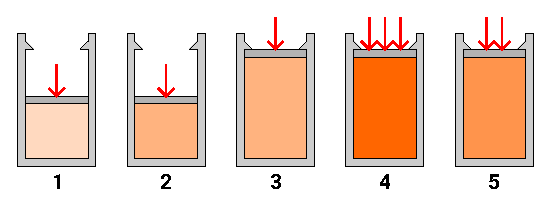
\includegraphics[scale=1.5]{resources/f1.eps}
\end{figure}

\textbf{\underline{Solución}:} \\

\underline{Datos provistos:} \\

\begin{equation*}
    \text{Agua}
\end{equation*}
\begin{equation*}
    P_1=5000[kPa]
\end{equation*}
\begin{equation*}
    T_1=80^\circ C
\end{equation*}
\begin{equation*}
    V=0.005134[m^3]
\end{equation*}
\begin{equation*}
    P_4=10000[kPa]
\end{equation*}
\begin{equation*}
    P_5=7000[kPa]
\end{equation*}
\begin{equation*}
    V_{max}=0.06366[m^3]
\end{equation*}

\underline{Estado 1}:\\
Extraemos la temperatura de ebullición para la presión dada, desde las tablas
termodinámicas:

\begin{equation*}
    T_{e}(5000[kPa])=263.99^\circ C
\end{equation*}

Como el agua esta a $80^\circ C$ se encuentra en la zona de liquido sub enfriado,
y considerando la baja compresibilidad de los líquidos, usamos el volumen
especifico y energía interna del liquido. 

\begin{equation*}
    \nu_1=0.001029[m^3/kg]
\end{equation*}
\begin{equation*}
    U_1=334.84[kJ/kg]
\end{equation*}

Conociendo el volumen total ($V$) y el volumen especifico ($\nu$), hallamos la
masa:

\begin{equation*}
    \nu=\frac{V}{m}\rightarrow
    m=\frac{V}{\nu_1}=\frac{0.005134}{0.001029}=4.9893[kg]
\end{equation*}

\begin{equation*}
\boxed{
    \begin{array}{l}
        T_1=80^\circ C \\
        P_1=5000[kPa] \\
        \nu_1=0.001029[m^3/kg] \\
        U_1=334.84[kJ/kg]
    \end{array}
}
\end{equation*}

\underline{Estado 2}:\\
La temperatura alcanza el punto de ebullición para la presión $P_1$:

\begin{equation*}
    T_{e}(5000[kPa])=263.99^\circ C
\end{equation*}

Extraemos el volumen especifico y energía interna para las condiciones actuales,
desde las tablas termodinámicas:

\begin{equation*}
    \nu_2=0.001286[m^3/kg]
\end{equation*}
\begin{equation*}
    U_2=1147,78[kJ/kg]
\end{equation*}

\begin{equation*}
\boxed{
    \begin{array}{l}
        T_2=263.99^\circ C \\
        P_2=5000[kPa] \\
        \nu_2=0.001286[m^3/kg] \\
        X_2=0 \\
        U_2=1147,78[kJ/kg]
    \end{array}
}
\end{equation*}

\underline{Estado 3}:\\
La presión y temperatura se mantienen constantes:

\begin{equation*}
    T_{e}(5000[kPa])=263.99^\circ C
\end{equation*}
\begin{equation*}
    \nu_v=0.03944[m^3/kg]
\end{equation*}
\begin{equation*}
    \nu_l=0.001286[m^3/kg]
\end{equation*}
\begin{equation*}
    U_v=2597.12[kJ/kg]
\end{equation*}
\begin{equation*}
    U_l=1147.78[kJ/kg]
\end{equation*}

Puede hallarse el volumen especifico a partir de la masa del agua y el volumen 
máximo, y por tanto el titulo.

\begin{equation*}
    \nu_3=\frac{V_{max}}{m}=\frac{0.06366}{4.9893}=0.012759[m^3/kg]
\end{equation*}
\begin{equation*}
    \nu=\nu_l+X(\nu_v-\nu_l)
\end{equation*}
\begin{equation*}
    X_3=\frac{\nu_3-\nu_l}{\nu_v-\nu_l}
    =\frac{0.012759-0.001286}{0.03944-0.001286}
    =0.3007
\end{equation*}

Se calcula la energía interna para el titulo hallado.

\begin{equation*}
    U_3=U_l+X_3(U_v-U_l)
\end{equation*}
\begin{equation*}
    U_3=1147.78+0.3007(2597.12-1147.78)=1583.6[kJ/kg]
\end{equation*}

\begin{equation*}
\boxed{
    \begin{array}{l}
        T_3=263.99^\circ C \\
        P_3=5000[kPa] \\
        \nu_3=0.012759[m^3/kg] \\
        X_3=0.3007 \\
        U_3=1583.6[kJ/kg]
    \end{array}
}
\end{equation*}

\underline{Estado 4}:\\
El volumen se mantiene constante, mientras que la presión incrementó a
$10000[kPa]$.

Extraemos la temperatura de ebullición para la presión dada, desde las tablas
termodinámicas:

\begin{equation*}
    T_{e}(10000[kPa])=311.06^\circ C
\end{equation*}
\begin{equation*}
    \nu_v=0.01803[m^3/kg]
\end{equation*}
\begin{equation*}
    \nu_l=0.001452[m^3/kg]
\end{equation*}
\begin{equation*}
    U_v=2544.41[kJ/kg]
\end{equation*}
\begin{equation*}
    U_l=1393.00[kJ/kg]
\end{equation*}

Hallamos el titulo para las condiciones dadas:

\begin{equation*}
    \nu=\nu_l+X(\nu_v-\nu_l)
\end{equation*}
\begin{equation*}
    X_4=\frac{\nu_4-\nu_l}{\nu_v-\nu_l}
    =\frac{0.012759-0.001452}{0.01803-0.001452}
    =0.6821
\end{equation*}

Se calcula la energía interna para el titulo hallado.

\begin{equation*}
    U_4=U_l+X_4(U_v-U_l)
\end{equation*}
\begin{equation*}
    U_4=1393.00+0.6821(2544.41-1393.00)=2178.3[kJ/kg]
\end{equation*}

\begin{equation*}
\boxed{
    \begin{array}{l}
        T_4=311.06^\circ C \\
        P_4=10000[kPa] \\
        \nu_4=0.012759[m^3/kg] \\
        X_4=0.6821 \\
        U_4=2178.3[kJ/kg]
    \end{array}
}
\end{equation*}

\underline{Estado 5}:\\
El volumen se mantiene constante, mientras que la presión se redujo a
$7000[kPa]$.

Extraemos la temperatura de ebullición para la presión dada, desde las tablas
termodinámicas:

\begin{equation*}
    T_{e}(7000[kPa])=285.88^\circ C
\end{equation*}
\begin{equation*}
    \nu_v=0.02737[m^3/kg]
\end{equation*}
\begin{equation*}
    \nu_l=0.001351[m^3/kg]
\end{equation*}
\begin{equation*}
    U_v=2580.48[kJ/kg]
\end{equation*}
\begin{equation*}
    U_l=1257.51[kJ/kg]
\end{equation*}

Hallamos el titulo para las condiciones dadas:

\begin{equation*}
    \nu=\nu_l+X(\nu_v-\nu_l)
\end{equation*}
\begin{equation*}
    X_5=\frac{\nu_5-\nu_l}{\nu_v-\nu_l}
    =\frac{0.012759-0.001351}{0.02737-0.001351}
    =0.4385
\end{equation*}

Se calcula la energía interna para el titulo hallado.

\begin{equation*}
    U_5=U_l+X_5(U_v-U_l)
\end{equation*}
\begin{equation*}
    U_5=1257.51+0.4385(2580.48-1257.51)=1837.6[kJ/kg]
\end{equation*}

\begin{equation*}
\boxed{
    \begin{array}{l}
        T_5=285.88^\circ C \\
        P_5=7000[kPa] \\
        \nu_5=0.012759[m^3/kg] \\
        X_5=0.4385 \\
        U_5=1837.6[kJ/kg]
    \end{array}
}
\end{equation*}

\underline{Trabajo}:\\
Se calcula el trabajo total:

\begin{equation*}
    W_{1\rightarrow 5}=W_{1\rightarrow 2}+W_{2\rightarrow 3}+
    W_{3\rightarrow 4}+W_{4\rightarrow 5}
\end{equation*}
\begin{equation*}
    W_{1\rightarrow 5}=\int_1^2 P_1 dv+\int_2^3 P_2 dv+0+0
\end{equation*}
\begin{equation*}
    W_{1\rightarrow 5}=P_1(V_2-V_1)+P_2(V_3-V_2)
\end{equation*}
\begin{equation*}
    W_{1\rightarrow 5}=P_1(V_3-V_1)
\end{equation*}
\begin{equation*}
    W_{1\rightarrow 5}=5000[kPa](0.06366[m^3]-0.005134[m^3])
\end{equation*}
\begin{equation*}
    W_{1\rightarrow 5}=292.63[kJ]
\end{equation*}

\underline{Calor intercambiado}:\\
Usando la primera ley de la termodinámica se obtiene el calor intercambiado:

\begin{equation*}
    \Delta U=Q-W
\end{equation*}
\begin{equation*}
    Q_{1\rightarrow 5}=\Delta U+W_{1\rightarrow 5}
\end{equation*}
\begin{equation*}
    Q_{1\rightarrow 5}=m(U_5-U_1)+W_{1\rightarrow 5}
\end{equation*}
\begin{equation*}
    Q_{1\rightarrow 5}=4.9893[kg](1837.6[kJ/kg]-334.83[kJ/kg])+292.63[kJ]
\end{equation*}
\begin{equation*}
    Q_{1\rightarrow 5}=7790.4[kJ]
\end{equation*}

\underline{Diagrama}:\\

\begin{figure}[!h]
\centering
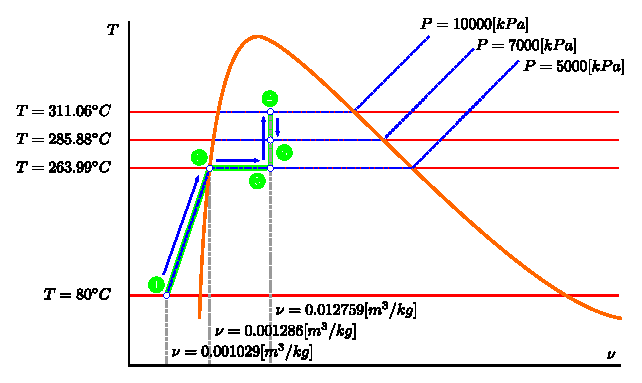
\includegraphics[scale=1.5]{resources/g1.eps}
\end{figure}

\newpage

\item Un cilindro con su embolo inicialmente contiene $1[m^3]$ de agua a
$100^\circ C$. El $70\%$ del volumen esta en estado liquido saturado y el resto
como vapor saturado. El embolo pesa $600[kg]$ y su diámetro es de $20[cm]$, la
presión atmosférica es de $100[kPa]$. Los pesos ejercen una presión de
$1.143[kg/cm^2]$. En el estado inicial hallar las masas de liquido y vapor. Se
entrega calor al agua hasta que su temperatura sea de $400^\circ C$. Halla el
trabajo realizado en el proceso.

\begin{figure}[!h]
\centering
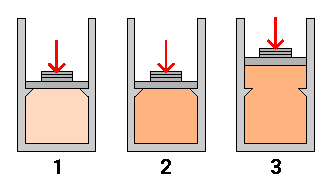
\includegraphics[scale=1.5]{resources/f2.eps}
\end{figure}

\textbf{\underline{Solución}:} \\

\underline{Datos provistos:} \\

\begin{equation*}
    \text{Agua}
\end{equation*}
\begin{equation*}
    V_1=1[m^3]
\end{equation*}
\begin{equation*}
    T_1=100^\circ C
\end{equation*}
\begin{equation*}
    0.7 V_l+0.3 V_v=V_1
\end{equation*}
\begin{equation*}
    m_E=600[kg]
\end{equation*}
\begin{equation*}
    d_E=20[cm]
\end{equation*}
\begin{equation*}
    P_{atm}=100[kPa]
\end{equation*}
\begin{equation*}
    \frac{m_P}{A}=1.143[kg/cm^2]
\end{equation*}
\begin{equation*}
    T_3=400^\circ C
\end{equation*}

\underline{Estado 1}:\\
Según tablas termodinámicas los valores para $100^\circ C$ son:

\begin{equation*}
    P_1=101.3[kPa]
\end{equation*}
\begin{equation*}
    \nu_v=1.67290[m^3/kg]
\end{equation*}
\begin{equation*}
    \nu_l=0.001044[m^3/kg]
\end{equation*}

Puede hallarse la masa a partir del porcentaje de vapor-liquido:

\begin{equation*}
    0.7V_l+0.3V_v=V_1
\end{equation*}
\begin{equation*}
    0.7\nu_l m+0.3\nu_v m=V_1
\end{equation*}
\begin{equation*}
    m(0.7\nu_l+0.3\nu_v)=V_1
\end{equation*}
\begin{equation*}
    m=\frac{V_1}{0.7\nu_l+0.3\nu_v}=1.9897[kg]
\end{equation*}

Y el volumen especifico y titulo es:

\begin{equation*}
    \nu_1=\frac{V_1}{m}=\frac{1}{1.9897}=0.5026[m^3/kg]
\end{equation*}
\begin{equation*}
    X_1=\frac{\nu_1-\nu_l}{\nu_v-\nu_l}
    =\frac{0.5026-0.001044}{1.67290-0.001044}
    =0.3
\end{equation*}

Por tanto las masas correspondientes son:

\begin{equation*}
    X=\frac{m_v}{m}\rightarrow
    m_v=X_1\,m=0.3(1.9897)=0.5969[kg]
\end{equation*}
\begin{equation*}
    m=m_v+m_l\rightarrow
    m_l=m-m_v=1.9897-0.5969=1.3927[kg]
\end{equation*}

\begin{equation*}
\boxed{
    \begin{array}{l}
        m_v=0.5969[kg] \\
        m_l=1.3927[kg] 
    \end{array}
}
\end{equation*}

\underline{Estado 3}:\\
Se calcula la presión resultante de las diferentes componentes:

\begin{equation*}
    P_3=P_{atm}+P_E+P_P
\end{equation*}
\begin{equation*}
    P_3=P_{atm}+\frac{F_E}{A_E}+\frac{F_P}{A_E}
\end{equation*}
\begin{equation*}
    P_3=P_{atm}+\frac{m_E\,g}{\pi r^2_E}+\frac{m_P\,g}{A_E}
\end{equation*}
\begin{equation*}
    P_3=P_{atm}+\frac{m_E\,g}{\pi r^2_E}+\frac{m_P\,g}{A_E}
\end{equation*}
\begin{equation*}
    P_3=100[kPa]+\frac{600[kg]9.8[m/s^2]}{\pi0.1^2[m^2]}\frac{1[kPa]}{1000[Pa]}+
    1.143(100^2)[kg/m^2]9.8[m/s^2]\frac{1[kPa]}{1000[Pa]}
\end{equation*}
\begin{equation*}
    P_3=399.18[kPa]
\end{equation*}

Para la presión obtenida se obtiene la temperatura de ebullición siguiente:

\begin{equation*}
    T_{e}(400[kPa])=143.63^\circ C
\end{equation*}

Por tanto, el agua se encuentra en zona de vapor sobre calentado, revisando en
tablas termodinámicas para $T=400^\circ C$ y $P=400[kPa]$ el valor del
volumen especifico es:

\begin{equation*}
    \nu_3=0.77262[m^3/kg]
\end{equation*}

Y se halla el volumen final:

\begin{equation*}
    \nu=\frac{V}{m}\rightarrow
    V=\nu\,m
\end{equation*}
\begin{equation*}
    V_3=0.77262(1.9897)[m^3]=1.5372[m^3]
\end{equation*}

Y finalmente se halla el trabajo realizado:

\begin{equation*}
    W_{1\rightarrow 3}=\int_1^3 P_3 dv
\end{equation*}
\begin{equation*}
    W_{1\rightarrow 3}=P_3(V_3-V_1)
\end{equation*}
\begin{equation*}
    W_{1\rightarrow 3}=399.19(1.5372-1)=214.46[kJ]
\end{equation*}

\underline{Diagrama}:\\

\begin{figure}[!h]
\centering
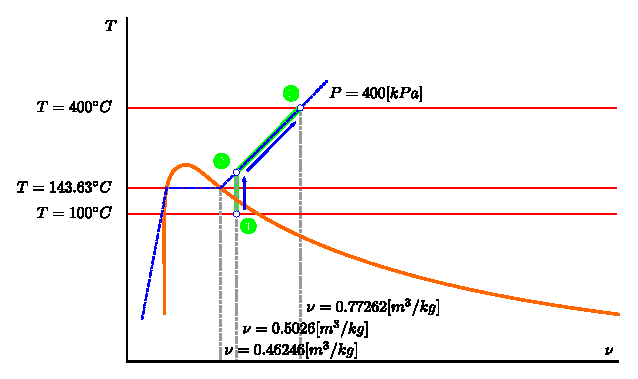
\includegraphics[scale=1.5]{resources/g2.eps}
\end{figure}

\newpage

\item Dentro de un cilindro con su embolo de área $0.01[m^2]$, se tiene $5[kg]$
de agua con un volumen de $0.5[m^3]$ a $500[kPa]$. Se entrega calor al agua y
cuando su volumen es de $0.8[m^3]$ encuentra una masa con un peso de $100[kg]$.
Se continua entregando calor hasta que todo este como vapor saturado. Hallar el
trabajo realizado en el proceso.

\begin{figure}[!h]
\centering
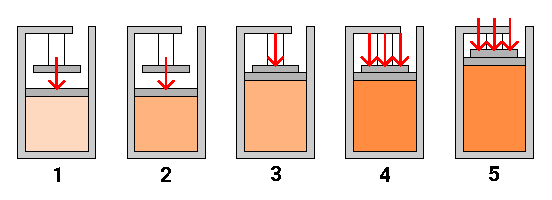
\includegraphics[scale=1.5]{resources/f3.eps}
\end{figure}

\textbf{\underline{Solución}:} \\

\underline{Datos provistos:} \\

\begin{equation*}
    \text{Agua}
\end{equation*}
\begin{equation*}
    A=0.01[m^2]
\end{equation*}
\begin{equation*}
    m=5[kg]
\end{equation*}
\begin{equation*}
    V_1=0.5[m^3]
\end{equation*}
\begin{equation*}
    P_1=500[kPa]
\end{equation*}
\begin{equation*}
    V_3=0.8[m^3]
\end{equation*}
\begin{equation*}
    m_p=100[kg]
\end{equation*}
\begin{equation*}
    X_5=1
\end{equation*}

\underline{Estado 1}:\\
Dado el volumen y la masa, se halla el volumen especifico:

\begin{equation*}
    \nu_1=\frac{V}{m}=\frac{0.5}{5}=0.1[m^3/kg]
\end{equation*}

Según tablas termodinámicas los valores para $500[kPa]$ son:

\begin{equation*}
    T_{e}(500[kPa])=151.86^\circ C
\end{equation*}
\begin{equation*}
    \nu_v=0.37489[m^3/kg]
\end{equation*}
\begin{equation*}
    \nu_l=0.001093[m^3/kg]
\end{equation*}

El titulo es:

\begin{equation*}
    X_1=\frac{\nu_1-\nu_l}{\nu_v-\nu_l}
    =\frac{0.01-0.001093}{0.37489-0.001093}
    =0.2646
\end{equation*}

\underline{Estado 3}:\\
Se calcula la presión con el peso adicional:

\begin{equation*}
    P_3=P_1+P_p
\end{equation*}
\begin{equation*}
    P_3=P_1+\frac{F}{A}
\end{equation*}
\begin{equation*}
    P_3=P_1+\frac{m_p\,g}{A}
\end{equation*}
\begin{equation*}
    P_3=500[kPa]+\frac{100[kg]9.8[m/s^2]}{0.01[m^2]}\frac{1[kPa]}{1000[Pa]}
    =598[kPa]
\end{equation*}

\underline{Estado 5}:\\
Extraemos la temperatura de ebullición para la presión dada, desde las tablas
termodinámicas:

\begin{equation*}
    T_{e}(600[kPa])=158.85^\circ C
\end{equation*}
\begin{equation*}
    \nu_v=0.31567[m^3/kg]
\end{equation*}
\begin{equation*}
    \nu_l=0.001101[m^3/kg]
\end{equation*}

Se calcula el volumen final para el titulo $X=1$:

\begin{equation*}
    \nu=\frac{V}{m}
\end{equation*}
\begin{equation*}
    V_5=m\nu_5=5(0.31567)=1.5783[m^3]
\end{equation*}

\underline{Trabajo}:\\
Se calcula el trabajo total:

\begin{equation*}
    W_{1\rightarrow 5}=W_{1\rightarrow 2}+W_{2\rightarrow 3}+
    W_{3\rightarrow 4}+W_{4\rightarrow 5}
\end{equation*}
\begin{equation*}
    W_{1\rightarrow 5}=0+W_{2\rightarrow 3}+0+W_{4\rightarrow 5}
\end{equation*}
\begin{equation*}
    W_{1\rightarrow 5}=\int_2^3 P_2 dv+\int_4^5 P_5 dv
\end{equation*}
\begin{equation*}
    W_{1\rightarrow 5}=P_2(V_3-V_2)+P_5(V_5-V_4)
\end{equation*}
\begin{equation*}
    W_{1\rightarrow 5}=500[kPa](0.8[m^3]-0.5[m^3])+598[kPa](1.5783[m^3]-0.8[m^3])
\end{equation*}
\begin{equation*}
    W_{1\rightarrow 5}=615.42[kJ]
\end{equation*}

\underline{Diagrama}:\\

\begin{figure}[!h]
\centering
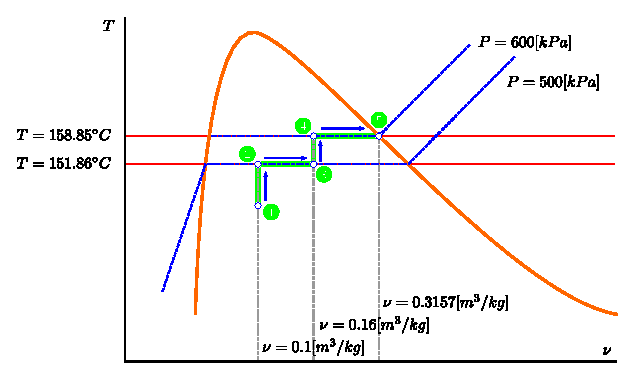
\includegraphics[scale=1.5]{resources/g3.eps}
\end{figure}

\newpage

\item Considere el esquema de la figura. El tanque $A$ tiene un volumen de
$100[lt]$ y contiene vapor saturado de $R134$ a $30^\circ C$. El cilindro $B$
inicialmente esta vacío. Se abre la válvula y el refrigerante fluye al cilindro
$B$. La presión para elevar el embolo es de $200[kPa]$. Se entrega calor de modo
que la temperatura este siempre a $30^\circ C$. El proceso termina cuando se
alcanza un estado uniforme en $A$ y en $B$. Hallar las masas finales en cada
recipiente y el trabajo realizado.

\begin{figure}[!h]
\centering
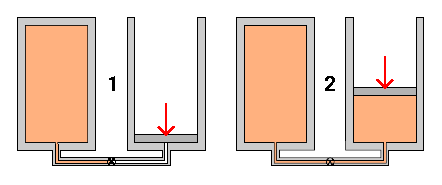
\includegraphics[scale=1.5]{resources/f4.eps}
\end{figure}

\textbf{\underline{Solución}:} \\

\underline{Datos provistos:} \\

\begin{equation*}
    \text{R134}
\end{equation*}
\begin{equation*}
    V_{1a}=100[lt]
\end{equation*}
\begin{equation*}
    X_{1a}=1
\end{equation*}
\begin{equation*}
    T_1=30^\circ C
\end{equation*}
\begin{equation*}
    P_{2b}=200[kPa]
\end{equation*}
\begin{equation*}
    T_2=30^\circ C
\end{equation*}

\underline{Estado 1}:\\
Según tablas termodinámicas los valores para $30^\circ C$ son:

\begin{equation*}
    P_{1a}=771.0[kPa]
\end{equation*}
\begin{equation*}
    \nu_v=0.02671[m^3/kg]
\end{equation*}
\begin{equation*}
    \nu_l=0.000843[m^3/kg]
\end{equation*}

Considerando el titulo $X=1$, se halla la masa:

\begin{equation*}
    \nu=\frac{V}{m}
\end{equation*}
\begin{equation*}
    m=\frac{V}{\nu}=\frac{100[lt]}{0.02671[m^3/kg]}\frac{0.001[m^3]}{1[lt]}
\end{equation*}
\begin{equation*}
    m=3.7439[kg]
\end{equation*}

\underline{Estado 2}:\\
Según tablas termodinámicas el valor para $P=200[kPa]$ y $T=30^\circ C$ es:

\begin{equation*}
    \nu_2=0.11889[m^3/kg]
\end{equation*}

Se calcula el volumen total:

\begin{equation*}
    \nu=\frac{V}{m}
\end{equation*}
\begin{equation*}
    V=m\nu_2=3.7439[kg]0.11889[m^3/kg]=0.4451[m^3]
\end{equation*}

Considerando que toda la sustancia esta en forma de vapor, se calcula la masa
en cada recipiente:

\begin{equation*}
    V_{2a}=0.1[m^3]
\end{equation*}
\begin{equation*}
    V_{2b}=V-V_{2a}=0.4451-0.1=0.34511[m^3]
\end{equation*}
\begin{equation*}
    m_{2a}=m\frac{V_{2a}}{V}=0.8411[kg]
\end{equation*}
\begin{equation*}
    m_{2b}=m\frac{V_{2b}}{V}=2.9028[kg]
\end{equation*}

\underline{Trabajo}:\\
Se calcula el trabajo total:

\begin{equation*}
    W_{1\rightarrow 2}=P_2(V_{2b}-V_{1b})
\end{equation*}
\begin{equation*}
    W_{1\rightarrow 2}=200[kPa](0.34511[m^3]-0[m^3])
\end{equation*}
\begin{equation*}
    W_{1\rightarrow 2}=69.023[kJ]
\end{equation*}

\end{enumerate}

\end{document}

